\scanpage{93}

\uline{Lemme 1} \quad $A$ anneau local noeth. \deleted{\unsure{quasi de}} \inserted{\deleted{\unsure{par hyp. un régulier}} quotient d'un régulier}
\deleted{formellement normal}, $t\in\unsure{\mathfrak r|r|\mathfrak m} A$ \inserted{un \unsure{élémt|élément} $A$-régulier}, on suppose
\deleted{$A/tA$ formellement normal} \inserted{le complété $t$-adique de $A$ normal} (à fortiori
$A$ \deleted{formellement} normal), et
$\dim A\geq 3$. Soit \deleted{$B$ fini sur $A$},
$B$ ``extension'' \inserted{finie} \uline{normale} \deleted{\unsure{génér.|de}} de $A$, et
supposons que $B/tB$ sur $A/tA$ soit
un rev. \deleted{\unsure{étale dans} le complément de l'origine} \inserted{\uline{trivial} hors de l'origine}.

\figure{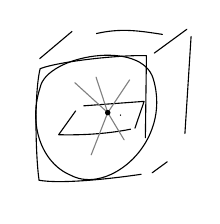
\begin{tikzpicture}[x=.27cm,y=.27cm,line cap=round,line join=round]
\draw (0,0) .. controls (-.15,1) and (-.25,4) .. (.05,5.25) .. controls (1,5.6) and (3.8,5.9) .. (5.05,5.86) -- (5,2);
\draw (0,0) .. controls (1,-.18) and (3.25,.05) .. (4.8,.28);
\draw (.03,5.72)--(1.55,7) (2.7,6.9)..controls(3.8,7.15)and(4.6,7.05)..(5.8,6.86) (5.42,5.98)--(6.95,7.1) (7.15,6.76)--(6.86,2.2) (5.32,.35)--(6.03,.87);
\draw (.92,2.14)--(1.72,3.26) (2.1,3.5)--(4.94,3.71)--(4.51,2.45) (4.3,2.4)..controls(2.7,2.08)and(1.2,2.14)..(.92,2.14);
\draw[gray] (3.23,3.18)--(1.68,4.59) (3.23,3.18)--(2.68,4.85) (3.23,3.18)--(4.26,4.72) (3.23,3.18)--(2.45,1.19) (3.23,3.18)--(4,1.9);
\fill (3.23,3.18) circle (.13); \fill (3.83,3.06) circle (.035);
\draw[thin] (.05,4.36) .. controls (.35,5.88) and (4.86,6.67) .. (5.38,4.74) .. controls (6.25,1.74) and (3.25,-.7) .. (1.5,.23) .. controls (.08,.82) and (-.51,2.68) .. (.05,4.36);
\end{tikzpicture}}

% slanted
\margin{Il suffit pour une \unsure{modification|rédaction|réduction} \unsure{minime|minima} de supposer que $B/tB$ coïncide dans le complémentaire de l'origine de $\unsure{\mathrm{Sp}}\,A/tA$ avec la restriction d'un rev. \uline{étale} de $A/tA$, \deleted{\unsure{ce dernier}} \deleted{\unsure{$A$}}}

Alors $B$ est un revêtement étale \deleted{hors de l'origine}

\uline{N.B.} L'hyp. implique que $B$ est étale sur $A$ en les pts de $V(t)-\text{origine}$ (grâce à la normalité de $A$ et $B$ \ldots\unsure{]|)} 

\deleted{Il revient \unsure{au même} de dire qu'il existe un}

\deleted{Comme} \deleted{Soit} $X=\mathrm{Spec}\,A$, \deleted{Soit} $X'=X-\{0\}$, $U$ l'ouvert des
pts de $\unsure{X|X'}$ en les quels $B$ est étale, alors
\deleted{[si $U\ne X$]} $(X-U)\cap V(t)\deleted{\unsure{=\varnothing}}\unsure{\subset|=}\{0\}$ et
$\dim(X-U)\leq 1$. On a un \unsure{revêtmt|revêtement} étale
\deleted{\unsure{de $X$}} \inserted{de} $U$, et il faut montrer qu'il se
prolonge en un rev. étale de $X$ \unsure{tt|\ensuremath{{}^{\prime}}}, \deleted{\unsure{un}}
\deleted{par le \unsure{compl.} dans les hyp. de} \deleted{\unsure{dim. et}}
Comme aux pts de $X-U$,
on a $\operatorname{prof}\mathscr O_{X,x}\geq 2$ [car $\dim\mathscr O_{X,x}\geq 2$,
et $\mathscr O_{X,x}$ est normal], cela signifie que

% slanted
\margin{condition des chaînes}

% archive sheet number: 92
